\documentclass{article}

\usepackage[final,nonatbib]{neurips_2023}

\usepackage[utf8]{inputenc}
\usepackage[T1]{fontenc}
\usepackage{hyperref}
\usepackage{url}
\usepackage{booktabs}
\usepackage{amsfonts}
\usepackage{nicefrac}
\usepackage{microtype}
\usepackage{xcolor}

\usepackage{graphicx}
\usepackage{caption}
\usepackage{subcaption}


\title{LOLCATS: Leveraging Obscure Lexical Conventions And Tenuous Synonyms in computer science research}


\author{%
  Kyle Roth \\
  DIRO \\
  Université de Montréal \\
  Montréal, QC, Canada \\
  \texttt{kyle.roth@umontreal.ca} \\
  \And
  Georges Bélanger\thanks{An especially cool guy.} \\
  Affiliation \\
  Address \\
  \texttt{email} \\
  \And
  Alex Fulleringer\thanks{An especially cool guy.} \\
  Affiliation \\
  Address \\
  \texttt{email} \\
}


\begin{document}


\maketitle


\begin{abstract}
  We did some stuff!
\end{abstract}


\section{Introduction}


We used the ART paper~\cite{paranjape2023art}.


\section{Background}


\section{Methodology}


\section{Experiments}


To effectively judge the usefulness of our method, we chose to evaluate on the abstractive summarization task. Unlike extractive summarization, in this task the summary is expected to be a concise representation that effectively communicates the key ideas in the text, rather than a composition of important phrases in the text. This is more like how humans generally summarize texts, and provides a stronger challenge for our method. We evaluated our method on the arXiv abstractive summarization dataset~\cite{cohan-etal-2018-discourse}. Texts in this dataset

\begin{figure}[h]
  \centering
  \begin{subfigure}{0.45\textwidth}
    \centering
    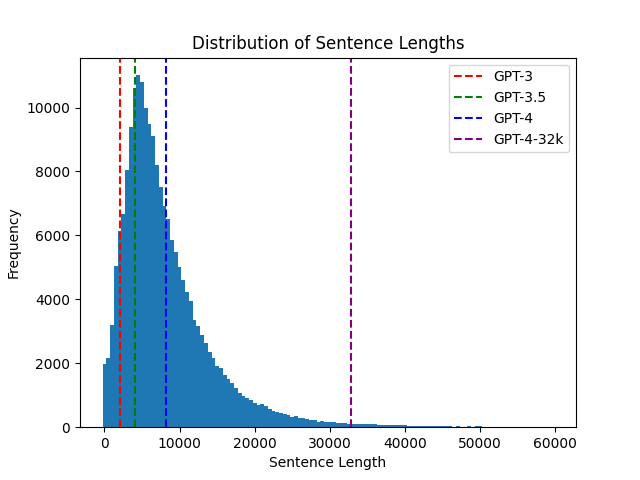
\includegraphics[width=\linewidth]{images/length_hist_train.png}
    \caption{Distribution of sentence lengths in the train set, by number of tokens. The sentence lengths have mean 8630.2, median 6883.0, minimum 0, and maximum 329071 (not visible).}\label{fig:train-hist}
  \end{subfigure}
  \hfill
  \begin{subfigure}{0.45\textwidth}
    \centering
    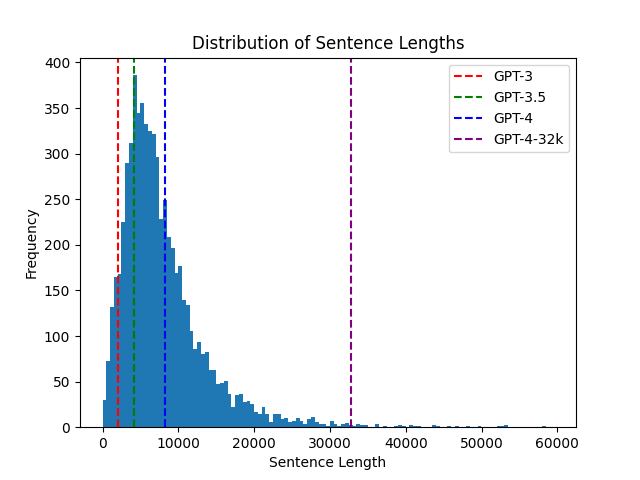
\includegraphics[width=\linewidth]{images/length_hist_validation.png}
    \caption{Distribution of sentence lengths in the validation set, by number of tokens. The sentence lengths have mean 8208.3, median 6871.5, minimum 244, and maximum 109442 (not visible).}\label{fig:val-hist}
  \end{subfigure}
  \caption{Distribution of sentence lengths in the train and validation sets.}\label{fig:length-hist}
\end{figure}


\section{Results}


\section{Conclusion}


\bibliographystyle{neurips}
\bibliography{main}


\end{document}
